\documentclass{exam}
\usepackage{../../commonheader}

%%% CHANGE THESE %%%%%%%%%%%%%%%%%%%%%%%%%%%%%%%%%%%%%%%%%%%%%%%%%%%%%%%%%%%%%%
\discnumber{5}
\title{\textsc{Orders of Growth}}
\date{March 7 to March 11, 2016}
%%%%%%%%%%%%%%%%%%%%%%%%%%%%%%%%%%%%%%%%%%%%%%%%%%%%%%%%%%%%%%%%%%%%%%%%%%%%%%%

\begin{document}
\maketitle
\rule{\textwidth}{0.15em}
\fontsize{12}{15}\selectfont

%%% INCLUDE TOPICS HERE %%%%%%%%%%%%%%%%%%%%%%%%%%%%%%%%%%%%%%%%%%%%%%%%%%%%%%%


%%% Question %%%

\begin{questions}
\begin{blocksection}
\question
In big-O notation, what is the runtime for \texttt{foo}?
\begin{parts}
\part
\begin{lstlisting}
def foo(n):
    for i in range(n):
        print('hello')
\end{lstlisting}
\begin{solution}[0.25in]
$O(n)$
\end{solution}

\part What's the runtime of \texttt{foo} if we change \texttt{range(n)}:
\begin{subparts}

\subpart To \texttt{range(n / 2)}?
\begin{solution}[0in]
$O(n)$
\end{solution}

\subpart To \texttt{range(10)}?
\begin{solution}[0in]
$O(1)$
\end{solution}

\subpart To \texttt{range(10000000)}?
\begin{solution}[0in]
$O(1)$
\end{solution}

\end{subparts}
\end{parts}
\end{blocksection}

\question What is the order of growth in time for the following functions? Use
big-O notation.
\begin{parts}

\part
\begin{lstlisting}
def strange_add(n):
    if n == 0:
        return 1
    else:
        return strange_add(n - 1) + strange_add(n - 1)
\end{lstlisting}
\begin{solution}[0.25in]
$O(2^n)$
\end{solution}

\part
\begin{lstlisting}
def stranger_add(n):
    if n < 3:
        return n
    elif n % 3 ==  0:
        return stranger_add(n - 1) + stranger_add(n - 2) + stranger_add(n - 3)
    else:
        return n
\end{lstlisting}
\begin{solution}[0.25in]
$O(n)$ is $n$ is a multiple of 3, otherwise $O(1)$.
\end{solution}

\newpage
\part
\begin{lstlisting}
def waffle(n):
    i = 0
    sum = 0
    while i < n:
        for j in range(50 * n):
            sum += 1
        i += 1
    return sum
\end{lstlisting}
\begin{solution}[0.25in]
$O(n^2)$
\end{solution}

\part
\begin{lstlisting}
def belgian_waffle(n):
    i = 0
    sum = 0
    while i < n:
        for j in range(n ** 2):
            sum += 1
        i += 1
    return sum
\end{lstlisting}
\begin{solution}[0.25in]
$O(n^3)$
\end{solution}

\part
\begin{lstlisting}
def pancake(n):
    if n ==  0:
        return n
    # Flip will always perform three operations and return -n.
    return flip(n) + pancake(n - 1) + pancake(n - 2)
\end{lstlisting}
\begin{solution}[0.25in]
$O(2^n)$
\end{solution}

\part
\begin{lstlisting}
def toast(n):
    i = 0
    j = 0
    stack = 0
    while i < n:
        stack += pancake(i)
        i += 1
    while j < n:
        stack += 1
        j += 1
    return stack
\end{lstlisting}
\begin{solution}[0.25in]
$O(n^3)$
\end{solution}

\end{parts}

\begin{blocksection}
\question Consider the following functions: 
\begin{lstlisting}
def hailstone(n):
   print(n)
   if n < 2:
    return
   if n % 2 == 0:
        hailstone(n // 2)
   else:
        hailstone((n * 3) + 1)

def fib(n):
   if n < 2:
      return n
   return fib(n - 1) + fib(n - 2)

def slow(n):
    i, j, k = 0, 0, 0
    while i < n:
        while j < n:
            while k < n:
                fib(k)
                k += 1
            fib(j)
            j += 1
        fib(i)
        i += 1

def foo(n, f):
    return n + f(500)
\end{lstlisting}
In big-O notation, describe the runtime for the following:
\begin{parts}
\part \texttt{foo(10, hailstone)}
\begin{solution}[0in]
$O(1)$
\end{solution}
\part \texttt{foo(3000, fib)}
\begin{solution}[0in]
$O(1)$
\end{solution}
\part \texttt{foo(99999999999, slow)}
\begin{solution}[0in]
$O(1)$
\end{solution}
\end{parts}

\end{blocksection}

\begin{blocksection}
\question \textbf{Fast Exponentiation:} in this problem, we will examine a
real-world algorithm used to improve the speed of calculating exponents.

\begin{parts}

\part First, express the runtime of the naive exponentiation algorithm in big-O
notation.
\begin{lstlisting}
def exp(b, n):
    if n == 0:
        return 1
    else:
        return b * exp(b, n - 1)
\end{lstlisting}
\begin{solution}[0.25in]
$O(n)$
\end{solution}

\part Now, express the runtime of the fast exponentiation algorithm in big-O
notation.
\begin{lstlisting}
def fast_exp(b, n):
    if n == 0:
        return 1
    elif n % 2 == 0:
        return square(fast_exp(b, n // 2))
    else:
        return b * fast_exp(b, n - 1)
\end{lstlisting}
\begin{solution}[0.25in]
$O(\log n)$
\end{solution}

\part What about this slightly modified version of \texttt{fast\char`_exp}?
\begin{lstlisting}
def fast_exp(b, n):
    for _ in range(50 * n):
        print("Killing time")
    if n == 0:
        return 1
    elif n % 2 == 0:
        return square(fast_exp(b, n // 2))
    else:
        return b * fast_exp(b, n - 1)
\end{lstlisting}
\begin{solution}[0.25in]
$O(n \log n)$
\end{solution}

\end{parts}
\end{blocksection}

\begin{blocksection}
\question \textbf{Mysterious loops:} What is the order of growth in time for the following functions? Use big-O notation.

\begin{parts}

\part
\begin{lstlisting}
def mystery(n):
    for i in range(n):
        while i % 2 != 0:
            print(i)
            i = i - 1
        print("Done")
\end{lstlisting}
\begin{solution}[0.25in]
$O(n)$
\end{solution}

\part
\begin{lstlisting}
def fun(n):
    for i in range(n):
        for j in range(n * n):
            if j == 4:
                return -1
            print("Fun!")
\end{lstlisting}
\begin{solution}[0.25in]
$O(1)$
\end{solution}
    
\end{parts}
\end{blocksection}

\begin{blocksection}
\question \textbf{Orders of Growth and Trees:} Assume we are using the non-mutable Tree implementation introduced in discussion. Consider the following function:
\begin{lstlisting}
def word_finder(t, n, word):
    if label(t) == word:
        n -= 1
        if n == 0:
            return True
    for child in children(t):
        if word_finder(child, n, word) == True:
            return True
    return False
\end{lstlisting}

\begin{parts}
\part What does this function do?  \newline
Hint: A path is a sequence of connected nodes. For example, here are four paths in the tree below: 1 $\rightarrow$ 2, 1 $\rightarrow$ 3 $\rightarrow$ 4, 1 $\rightarrow$ 3 $\rightarrow$ 5, 1 $\rightarrow$ 3 $\rightarrow$ 6 

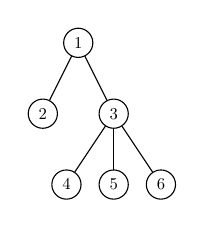
\begin{tikzpicture}[scale=0.6, transform shape]
\tikzstyle{level 2}=[sibling distance=10mm]
    \node [circle, draw] (z){$1$}
        child {node [circle, draw] (a) {$2$}}
        child {node [circle, draw] (d) {$3$}
            child {node [circle, draw] (g) {$4$}}
            child {node [circle, draw] (e) {$5$}}
            child {node [circle, draw] (f) {$6$}}
        };
\end{tikzpicture}
\begin{solution}[0.25in]
This function take a Tree \texttt{t}, an integer \texttt{n}, and a string
\texttt{word} in as input. Then, \texttt{word\char`_finder} returns True if the
word appears as a label in the Tree \texttt{n}-times and False otherwise.
\end{solution}

\part If a tree has $n$ total nodes, what is the total runtime for all searches
in big-O notation?
\begin{solution}[0.25in]
$O(n)$
\end{solution}

\end{parts}

\end{blocksection}

\begin{blocksection}
\question \textbf{Orders of Growth and Linked Lists:} Consider the following
linked list function:
\begin{lstlisting}
def insert_at_end(lst, x):
    if lst.rest is Link.empty:
        lst.rest = Link(x)
    else:
        insert_at_end(lst.rest, x)
\end{lstlisting}

\begin{parts}
\part What does this function do?
\begin{solution}[0.25in]
    Inserts a value \texttt{x} at the end of linked list \texttt{lst}.
\end{solution}
\part Say we want to repeatedly insert some numbers into the end of a linked
list:
\begin{lstlisting}
def insert_many(lst, n):
    for i in range(n):
        insert_at_end(lst, i)
\end{lstlisting}
\begin{subparts}

\subpart Assume \texttt{lst} is initially length 1. How long will it take to do
the first insertion? The second? The $n$th?
\begin{solution}[0.25in]
Notice that the list gets longer with each insertion, so each operation will
make it harder to do the next.
Therefore, the first insertion will take about 1 unit of time. The second will
take about twice as long, at two units of time. The $n$th insertion will take
$n$ units of time.
\end{solution}

\subpart In big-O notation, What is the total runtime to do all the inserts?
(total runtime of \texttt{insert\char`_many})
\begin{solution}[0.25in]
The total runtime will be the sum of all the inserts: 1 + 2 + 3 + \ldots + $n$ =
$\frac{n (n + 1)}{2}$ = $O(n^{2})$
\end{solution}

\end{subparts}

\end{parts}
\end{blocksection}

\end{questions}

%%%%%%%%%%%%%%%%%%%%%%%%%%%%%%%%%%%%%%%%%%%%%%%%%%%%%%%%%%%%%%%%%%%%%%%%%%%%%%%

\end{document}
